\begin{figure}
\begin{center}
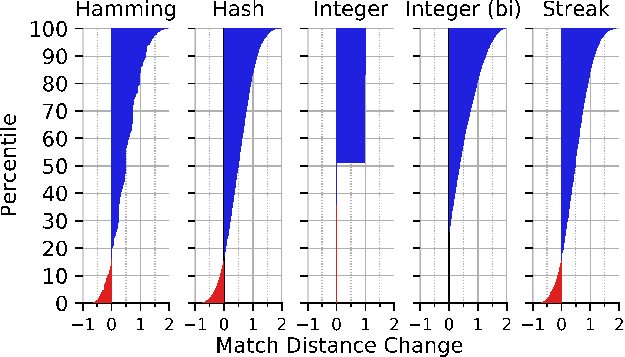
\includegraphics[width=\linewidth]{img/detour_difference/bitweight=0dot5+seed=1+title=low-triplet-analysis+_data_hathash_hash=6b0749ef97a58721+_script_fullcat_hash=2ded962cad675fe3+ext=}
\caption{
Cumulative distributions of sampled detour difference values.
Each distribution visualization arranges individually sampled observations (thin horizontal bars) vertically in descending order.
The $y$ axis can be interpreted as ranging from the \nth{0} percentile of outcomes (bottom) to \nth{100} percentile (top) with horizontal bar width showing the detour difference at a certain percentile.
A positive value (colored blue) indicates that total distance increased with the addition of an intermediate stop.
A value of exactly 0 indicates an intermediate stop had no effect on total distance.
A negative value (colored red) indicates violation of the triangle inequality: taking an intermediate stop reduced the total distance traveled.
}
\label{fig:detour_difference_supp}

\end{center}
\end{figure}
